%%%%%%%%%%%%%%%%%%%%%%%%%%%%%%%%%%%%%%%%%
% Beamer Presentation
% LaTeX Template
% Version 1.0 (10/11/12)
%
% This template has been downloaded from:
% http://www.LaTeXTemplates.com
%
% License:
% CC BY-NC-SA 3.0 (http://creativecommons.org/licenses/by-nc-sa/3.0/)
%
%%%%%%%%%%%%%%%%%%%%%%%%%%%%%%%%%%%%%%%%%

%----------------------------------------------------------------------------------------
%	PACKAGES AND THEMES
%----------------------------------------------------------------------------------------

\documentclass{beamer}


\mode<presentation> {

% The Beamer class comes with a number of default slide themes
% which change the colors and layouts of slides. Below this is a list
% of all the themes, uncomment each in turn to see what they look like.

%\usetheme{default}
%\usetheme{AnnArbor}
%\usetheme{Antibes}
%\usetheme{Bergen}
%\usetheme{Berkeley}
%\usetheme{Berlin}
%\usetheme{Boadilla}
%\usetheme{CambridgeUS}
%\usetheme{Copenhagen}
%\usetheme{Darmstadt}
%\usetheme{Dresden}
%\usetheme{Frankfurt}
%\usetheme{Goettingen}
%\usetheme{Hannover}
%\usetheme{Ilmenau}
%\usetheme{JuanLesPins}
%\usetheme{Luebeck}
\usetheme{Madrid}
%\usetheme{Malmoe}
%\usetheme{Marburg}
%\usetheme{Montpellier}
%\usetheme{PaloAlto}
%\usetheme{Pittsburgh}
%\usetheme{Rochester}
%\usetheme{Singapore}
%\usetheme{Szeged}
%\usetheme{Warsaw}

% As well as themes, the Beamer class has a number of color themes
% for any slide theme. Uncomment each of these in turn to see how it
% changes the colors of your current slide theme.

%\usecolortheme{albatross}
%\usecolortheme{beaver}
%\usecolortheme{beetle}
%\usecolortheme{crane}
%\usecolortheme{dolphin}
%\usecolortheme{dove}
%\usecolortheme{fly}
%\usecolortheme{lily}
%\usecolortheme{orchid}
%\usecolortheme{rose}
%\usecolortheme{seagull}
%\usecolortheme{seahorse}
%\usecolortheme{whale}
%\usecolortheme{wolverine}

%\setbeamertemplate{footline} % To remove the footer line in all slides uncomment this line
%\setbeamertemplate{footline}[page number] % To replace the footer line in all slides with a simple slide count uncomment this line

%\setbeamertemplate{navigation symbols}{} % To remove the navigation symbols from the bottom of all slides uncomment this line
}

\usepackage{macros}
%\usepackage{biblatex}
%\addbibresource{ijcai17.bib}
%\usepackage{natbib}
%\usepackage[round]{natbib}
%\usepackage[comma,numbers,sort&compress]{natbib}

%----------------------------------------------------------------------------------------
%	TITLE PAGE
%----------------------------------------------------------------------------------------

\title[Thresholding Bandits with Augmented UCB]{Thresholding Bandits with Augmented UCB} % The short title appears at the bottom of every slide, the full title is only on the title page

\author{Subhojyoti Mukherjee\\ Roll No: CS15S300 \\ Guide: Dr. Balaraman Ravindran \\ Co-Guide: Dr. Nandan Sudarsanam} % Your name
\institute[IIT Madras] % Your institution as it will appear on the bottom of every slide, may be shorthand to save space
{
IIT Madras \\ % Your institution for the title page
\medskip
%\textit{john@smith.com} % Your email address
}
\date{\today} % Date, can be changed to a custom date

\begin{document}
\nocite{*}
\begin{frame}
\titlepage % Print the title page as the first slide
\end{frame}

\begin{frame}
\frametitle{Overview} % Table of contents slide, comment this block out to remove it
\tableofcontents % Throughout your presentation, if you choose to use \section{} and \subsection{} commands, these will automatically be printed on this slide as an overview of your presentation
\end{frame}

%----------------------------------------------------------------------------------------
%	PRESENTATION SLIDES
%----------------------------------------------------------------------------------------


%\section{Introduction}
%\begin{frame}
\frametitle{Introduction to bandits}
\begin{itemize}
\item<1-> The bandit problem is a sequential decision making process where at each timestep we have to choose one action or arm from a set of arms.
\item<2-> There is a specific reward distribution attached to each arm.  After pulling an arm we receive a reward (without delay) from the reward distribution specific to the arm. 
\item<3-> After (say) pulling each arm once, we are presented with an \emph{exploration-exploitation}  trade-off, that is whether to continue to pull the arm for which we have observed the highest estimated reward till now(exploitation) or to explore a new arm(exploration). 
\item<4-> If we become too greedy and always exploit, we may miss the chance of actually finding the optimal arm and get stuck with a sub-optimal arm.
\end{itemize}
\end{frame}




\section{Stochastic Multi-Armed Bandit Problem}
\begin{frame}
\frametitle{Stochastic Multi-Armed Bandit Problem (SMAB)}
\begin{itemize}
\item<1-> The thresholding bandit problem falls under the broad area of stochastic multi-armed bandit problem.
\item<2-> In SMAB problem, we are presented with a finite set of actions or arms belonging to set $A$ such that $|A|=K$. 
\item<3-> The rewards for each of the arms are identical and independent random variables drawn from distribution specific to the arm.
\item<4-> The learner does not know the mean of the distributions, denoted by $r_{i},\forall i\in A$ or  the variance denoted by $\sigma_i^2$. 
\item<5-> The distributions for each of the arms are fixed throughout the time horizon denoted by $T$. 
\end{itemize}
\end{frame}




\section{Problem Definition}
\begin{frame}
\frametitle{Problem Definition}
\begin{itemize}
\item<1-> The primary aim in the thresholding bandit problem (TBP) is to identify the arms whose mean of the reward distribution is above a particular threshold $\tau$ given as input.
\item<2-> The above goal has to be achieved within $T$ timesteps of exploration and this is termed as a fixed-budget problem.
\item<3-> At the end of the given $T$ timesteps the learner must recommend a set of arms which (according to it) are the arms having reward mean above $\tau$.
\end{itemize}
\end{frame}

\begin{frame}
\frametitle{Problem Definition}
\begin{itemize}
\item<1-> We define the set $S_{\tau}=\lbrace i\in \mathcal{A}: r_{i}\geq \tau \rbrace$. 
%Note that, $S_\tau$ is the set of all arms whose reward mean is greater than $\tau$. Let 
\item<2-> $S_\tau^c$ denote the complement of $S_\tau$, i.e.,  $S_{\tau}^{c}=\lbrace i\in \mathcal{A}: r_{i} < \tau \rbrace$. 
\item<3-> Let $\hat{S}_{\tau}$ denote the recommendation of a learning algorithm after $T$ time units of exploration, while $\hat{S}_{\tau}^c$ denotes its complement.

%\item<4-> The performance of the learning agent is measured by the accuracy with which it can classify the arms into $S_{\tau}$ and $S_{\tau}^{c}$ after time horizon $T$. Equivalently, the \emph{loss} $\mathcal{L}(T)$ is defined as
%\begin{align*}
%\Ls (T) = \mathbb{I}\big(\lbrace S_{\tau}\cap \hat{S}_{\tau}^{c}\neq \emptyset\rbrace    \cup    \lbrace\hat{S}_{\tau}\cap S_{\tau}^{c}\neq \emptyset\rbrace\big).
%\end{align*}			

\item<4-> The goal of the learning agent is to minimize the expected loss:
\begin{align*}
\Ex[\Ls(T)] &= \Pb\big(\lbrace S_{\tau}\cap \hat{S}_{\tau}^{c} \neq \emptyset \rbrace  \cup   \lbrace \hat{S}_{\tau}\cap S_{\tau}^{c} \neq \emptyset\rbrace\big) \\
& = 1 - \Pb\big(\lbrace \hat{S}_{\tau}\cap {S}_{\tau}^{c} = \emptyset \rbrace \cap \lbrace \hat{S}_{\tau}^c \cap {S}_{\tau} = \emptyset \rbrace \big )
\end{align*}
\end{itemize}
\end{frame}

\begin{frame}
\frametitle{Challenges in the TBP Settings}
\begin{itemize}
\item<1-> The more number of arms' means are closer to the threshold the harder is to discriminate between them.
\item<2-> The lesser the budget is, the harder the problem becomes.
\item<3-> The higher the variance of the arms' the more difficult is to discriminate.
\end{itemize}
\end{frame}


\begin{frame}
\frametitle{Some practical applications}
\begin{itemize}
\item<1-> Selecting the best channels (out of several existing channels) for mobile communications in a very short duration whose qualities are above an acceptable threshold (see \cite{audibert2010best}).
\item<2-> Selecting a small set of best workers (out of a very large pool of workers) whose productivity is above a threshold.
\item<3-> In anomaly detection and classification (see {Locatelli et al. (2016)}).
\end{itemize}
\end{frame}

%The above TBP formulation has several applications, for instance, from areas ranging from anomaly detection and classification (see  \citet{locatelli2016optimal}) to industrial applications as well as in mobile communications (see \citet{audibert2010best})  where the users are to be allocated only those channels whose quality is above an acceptable threshold.

\section{Contribution}
\begin{frame}
\frametitle{Contribution}
\begin{itemize}
\item<1-> We propose the Augmented UCB (AugUCB) \cite{DBLP:journals/corr/MukherjeeNSR17} algorithm for the fixed-budget TBP setting.
\item<2-> AugUCB takes into account the empirical variances of the arms along with mean estimates.
\item<3-> It is the first variance-based arm elimination algorithm for the considered TBP settings. 
\item<4-> It address an open problem discussed in \cite{auer2010ucb} of designing an algorithm that can eliminate arms based on variance estimates.
\item<5-> It is the first algorithm on the larger pure exploration setting which uses empirical variance estimates along with arm elimination with a new problem complexity.
\end{itemize}
\end{frame}


%Our theoretical contribution comprises proving an upper bound on the expected loss incurred by AugUCB (Theorem~\ref{Result:Theorem:1}).
%In Table \ref{tab:regret-bds} we compare the upper bound on the losses incurred by the various algorithms, including AugUCB. The terms $H_1, H_2$, $H_{CSAR,2}, H_{\sigma,1}$ and $H_{\sigma,2}$ represent various problem complexities, and are as defined in Section~\ref{results}. From Section~\ref{results} we note that, for all $K\ge8$, we have
%\begin{align*}
%\log\left(K\log K\right) H_{\sigma,2} > \log(2K) H_{\sigma,2} \ge H_{\sigma,1}.
%\end{align*}
%
%Thus, it follows that the upper bound for UCBEV is better than that for AugUCB. However, implementation of UCBEV algorithm requires $H_{\sigma,1}$ as input, whose computation is not realistic in practice. In contrast, our AugUCB algorithm requires no such complexity factor as input. Proceeding with the comparisons, we emphasize that the upper bound for  AugUCB is, in fact, not comparable with that of APT and CSAR; this is because the complexity term $H_{\sigma,2}$ is not explicitly comparable with either $H_1$ or $H_{CSAR,2}$. However, through extensive simulation experiments we find that AugUCB significantly outperforms both APT, CSAR and other non variance-based algorithms. AugUCB also outperforms UCBEV under explorations where non-optimal values of $H_{\sigma,1}$  are used. In particular, we consider experimental scenarios comprising large number of arms, with the variances of arms in $S_\tau$ being large. AugUCB, being variance based, exhibits superior performance under these settings.  
%%




\section{Previous Works}
\begin{frame}
\frametitle{Previous Works}
\begin{itemize}
\item<1-> The Anytime Parameter Free (APT) [{Locatelli et al. (2016)}] algorithm was proposed for TBP setting in ICML 2016. 
\item<2-> This algorithm uses only mean estimation to find the $S_{\tau}$. 
\item<3-> Theoretically they proved this algorithm to be almost optimal when only mean estimation is used as a metric of comparison.
\item<4-> Empirically it outperformed other state-of-the-art algorithms which were modified to perform in the TBP setting.  
\end{itemize}
\end{frame}

\begin{frame}
\frametitle{APT Algorithm}
\begin{algorithm}[H]
\caption{APT}
\begin{algorithmic}[1]
\State {\bf Input:} Time horizon $T$, threshold $\tau$, tolerance factor $\epsilon\geq 0$
\State Pull each arm once
\vspace{-3mm}
\State \For{$t=K+1,..,T$}
\State Pull arm $j\in\argmin_{i\in A}\Big\lbrace \left(|\hat{r}_{i} - \tau | + \epsilon\right)\sqrt{n_i}\Big\rbrace$ and observe the reward for arm $j$.
\EndFor
\State \textbf{Output:} $\hat{S}_{\tau}=\lbrace i: \hat{r}_{i}\geq \tau \rbrace$.
\end{algorithmic}
\end{algorithm}
\end{frame}

\begin{frame}
\frametitle{Previous Works (Pure Exploration)}
\begin{itemize}
\item<1-> The TBP problem also falls within the larger area called the Pure Exploration problem.
\item<2-> In pure exploration problems the learner has to output a set of recommendations either with high confidence (fixed confidence) or after a specified number of rounds (fixed budget).
\item<3-> Our considered TBP is a fixed budget pure exploration problem.
\item<4-> Both APT and AugUCB reuses several ideas from Pure exploration problem. 
\end{itemize}
\end{frame}

\begin{frame}
\frametitle{Previous Works (Diagram)}
\centering
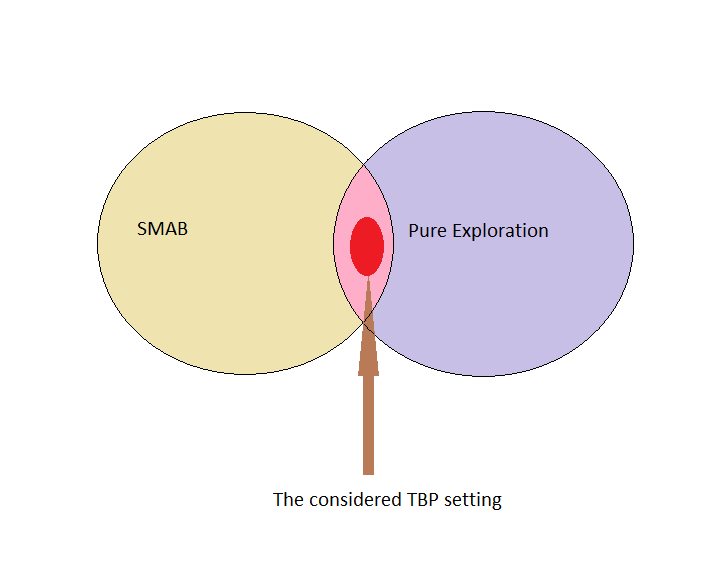
\includegraphics[scale=0.5]{img/Settings2.png}
\end{frame}

\begin{frame}
\frametitle{Approach of UCB-Improved (UCB-Imp)}
\begin{itemize}
\item<1-> There is a strong relation between UCB-Imp \cite{auer2010ucb} and AugUCB where the former is used to find \emph{a single optimal arm as quickly as possible}.
\item<2-> The basic idea of UCB-Improved is to divide the horizon into phases or rounds and initialize parameters.
\item<3-> Pull all surviving arms equal number of times during a round.
\item<4-> At the end of the round eliminate some sub-optimal arms (as judged by learner) based on elimination criteria.
\item<5-> Reset parameters and proceed to next round.
%\item<5-> UCB-Imp achieves a gap-independent regret bound of $O\left( \sqrt{KT\log K}\right)$ and gap-dependent bound of $O\left( \dfrac{K \log (T\Delta^2)}{\Delta}\right)$.
\end{itemize}
\end{frame}

\begin{frame}
\frametitle{UCB-Improved (\cite{auer2010ucb})}
\begin{algorithm}[H]
\caption{UCB-Improved}
\small
\begin{algorithmic}[1]
\State {\bf Input:} Time horizon $T$
\State {\bf Initialization:} Set $B_{0}:=A$ and ${\epsilon}_{0}:=1$.
\For{$m=0,1,..\big \lfloor \dfrac{1}{2}\log_{2} \dfrac{T}{e}\big\rfloor$}	
\State Pull each arm in $B_m$, $n_{m}=\bigg\lceil\dfrac{2\log{( T{\epsilon}_{m}^{2})}}{{\epsilon}_{m}}\bigg\rceil$ number of times.
%so that the total  it has been pulled is
\ArmElim
\State For each $i \in B_{m}$, delete arm ${i}$ from $B_{m}$ if,
\begin{align*}
\hat{r}_{i} + \sqrt{\dfrac{\log{(T{\epsilon}_{m}^{2})}}{2 n_{m}}}  < \max_{{j}\in B_{m}}\bigg\lbrace\hat{r}_{j} -\sqrt{\dfrac{\log{( T{\epsilon}_{m}^{2})}}{2 n_{m}}} \bigg\rbrace
\end{align*}
\EndArmElim
%\ResParam
\State Set ${\epsilon}_{m+1}:=\dfrac{{\epsilon}_{m}}{2}$, Set $B_{m+1}:=B_{m}$
%\EndResParam
\State Stop if $|B_{m}|=1$ and pull ${i}\in B_{m}$ till $n$ is reached.
\EndFor
\end{algorithmic}
\end{algorithm}
\end{frame}

\begin{frame}
\frametitle{Some technical details of UCB-Improved}
\begin{itemize}
\item<1-> We do not know the true means $r_i ,\forall i\in A$ of the distributions so we estimate it by the ${\epsilon}$ by initializing it from $1$.
\item<2-> All rewards are assume to be bounded between $[0,1]$ and so $\Delta_{i} = (r^* - r_i)\in [0,1],\forall i\in A$ as well.
\item<3-> UCB-Improved has fixed confidence interval  $c_{m}=\sqrt{\dfrac{\log{(T{\epsilon}_{m}^{2})}}{2 n_{m}}}$ for all arms in a particular phase.
\item<4-> $c_m$ ensures that whenever ${\epsilon}_{m}<\dfrac{\Delta_i}{2}$ in the $m$-th round, the arm $i$ gets eliminated.
\end{itemize}
\end{frame}

\section{AugUCB}
\begin{frame}
\frametitle{AugUCB algorithm}
\begin{figure}
%\caption{AugUCB Flowchart}
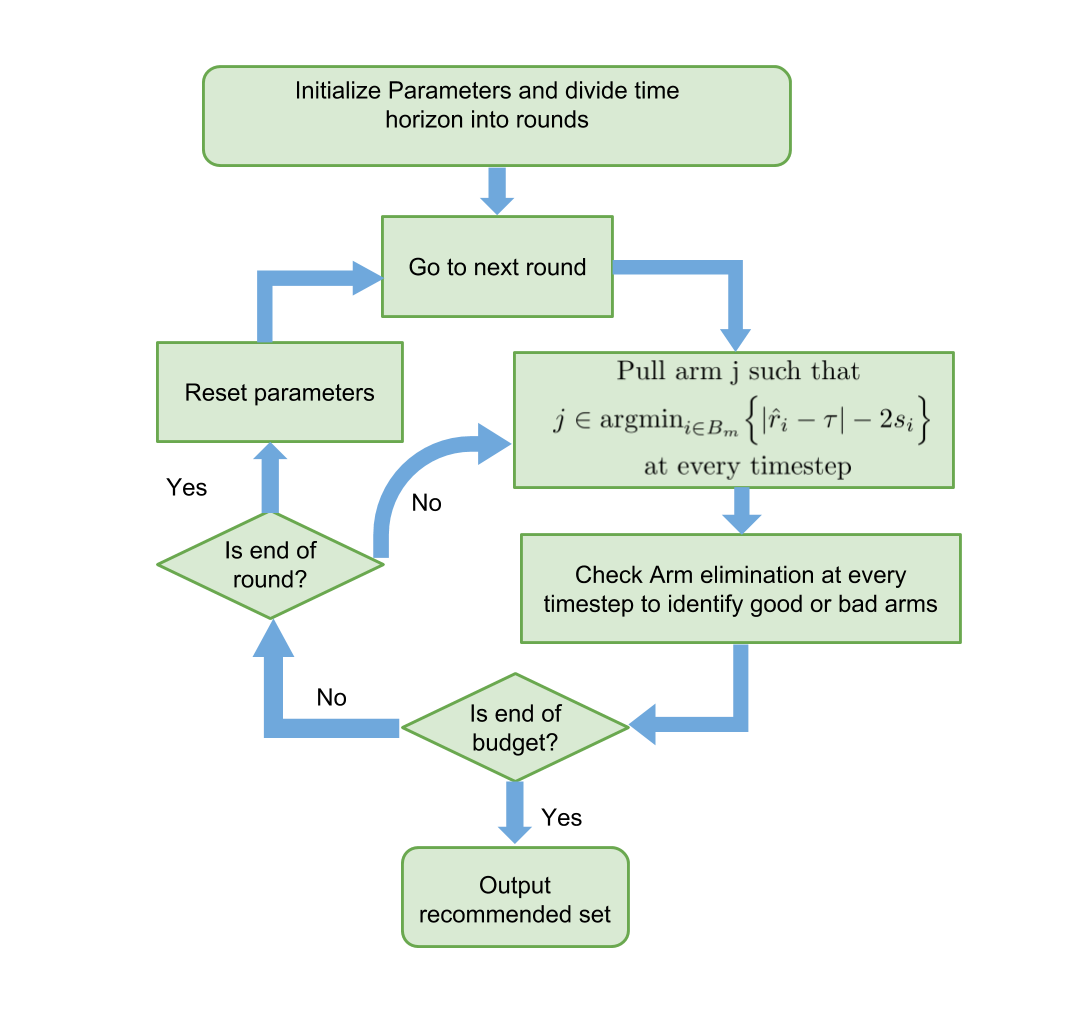
\includegraphics[scale=0.24]{img/AugUCB_flow.png}
\end{figure}
\end{frame}



\begin{frame}
\frametitle{AugUCB algorithm (Intuition, Arm pulling)}
\begin{itemize}
%\item We define $\Delta_i = |r_i - \tau| $ . 
\item Like UCB-Imp, AugUCB also divides the time budget $T$ into rounds.
\item At every timestep we pull arm j s.t. $j\in\argmin_{i\in B_{m}}\Big\lbrace |\hat{r}_{i} - \tau | - 2s_{i}\Big\rbrace$ (like APT). 
\end{itemize}

\begin{figure}
%\caption{AugUCB Intuition (Arm pulling)}
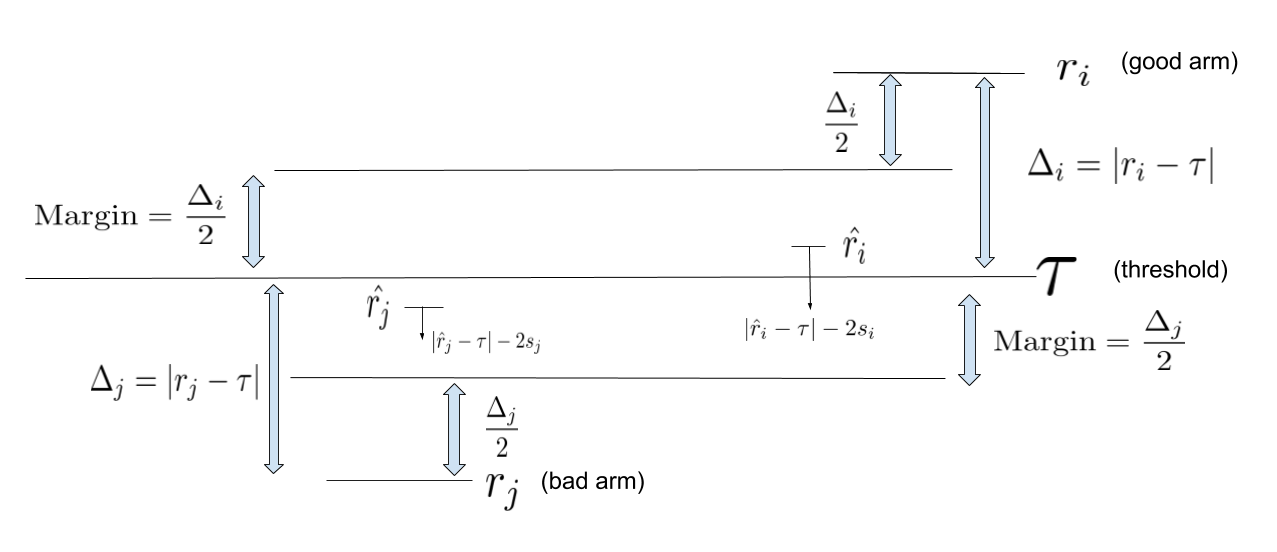
\includegraphics[scale=0.278]{img/SeminarThresholdBandit.png}
\end{figure}
\end{frame}

\begin{frame}
\frametitle{AugUCB algorithm (Intuition, Arm Elimination)}
\begin{itemize}
\item It is risky to eliminate arm $i$ while $\hat{r}_i$ is inside \emph{Margin}. 
\item Confidence interval $s_i$ will make sure arm $i$ is not eliminated while inside Margin with a high probability. 
\end{itemize}

\begin{figure}
%\caption{AugUCB Intuition (Arm Elimination)}
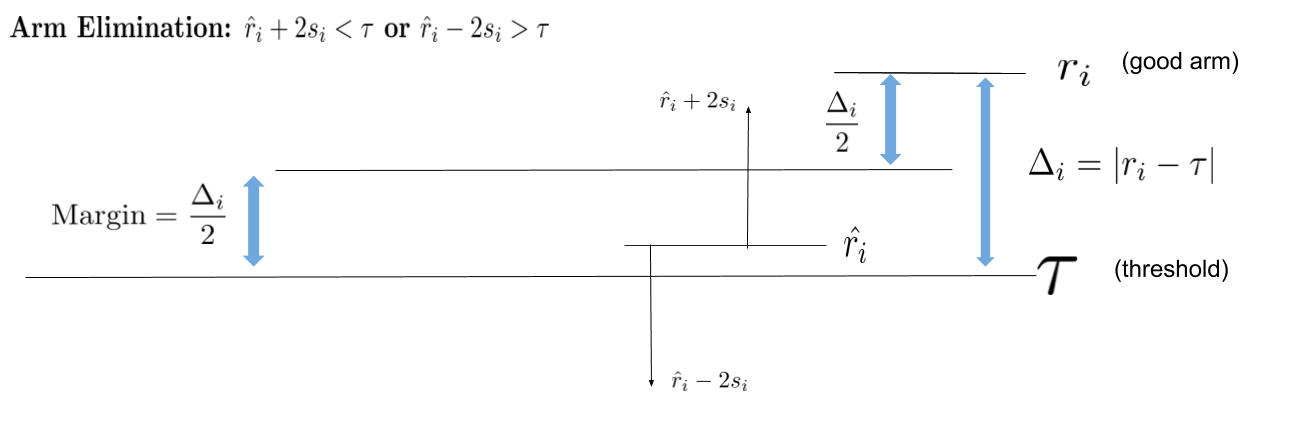
\includegraphics[scale=0.278]{img/ArmElim1.png}
\end{figure}
\end{frame}

\begin{frame}
\frametitle{AugUCB algorithm (Intuition, Arm Elimination)}
\begin{figure}
%\caption{AugUCB Intuition (Arm Elimination)}
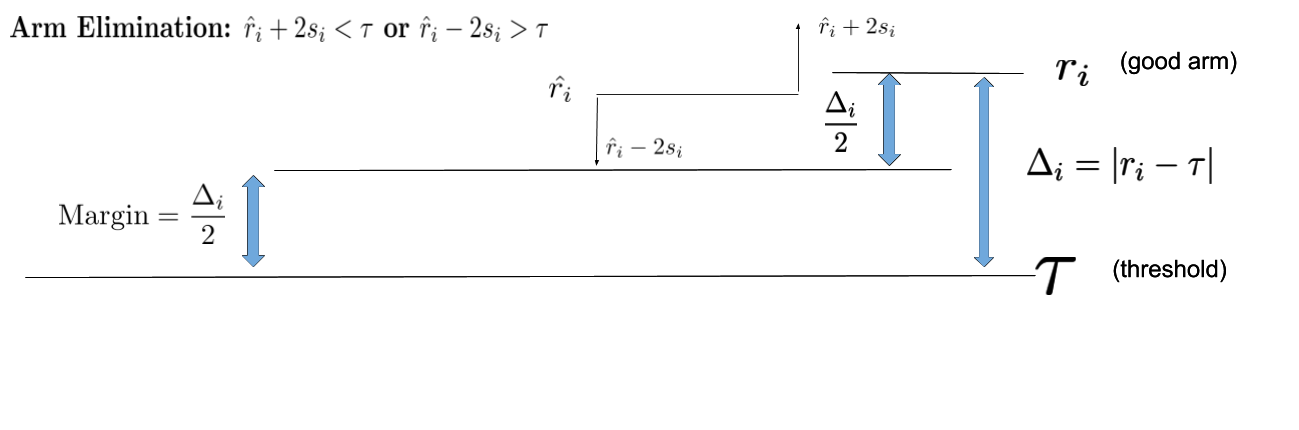
\includegraphics[scale=0.278]{img/ArmElim2.png}
\end{figure}
\end{frame}

%\begin{frame}
%\frametitle{AugUCB algorithm}
%\begin{figure}
%%\caption{AugUCB Flowchart}
%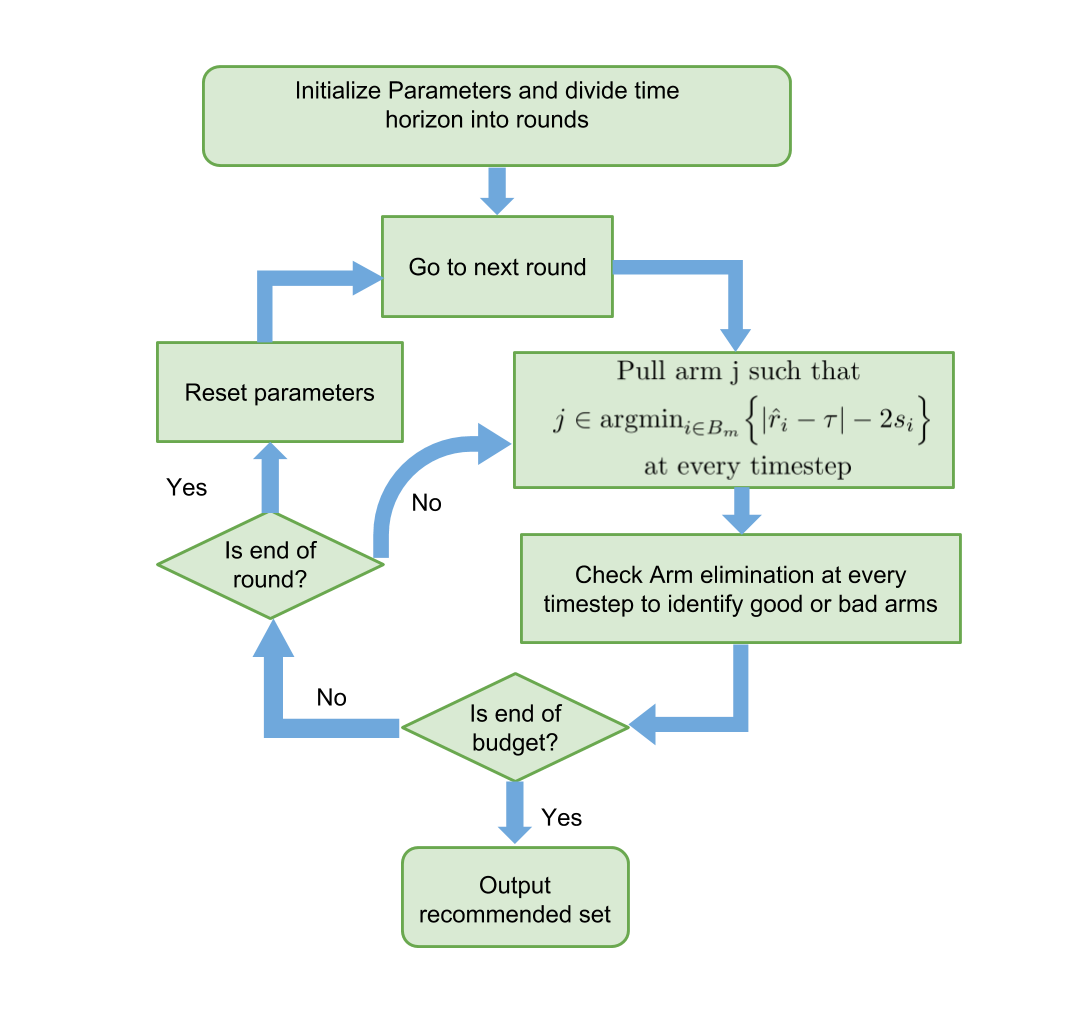
\includegraphics[scale=0.24]{img/AugUCB_flow.png}
%\end{figure}
%\end{frame}


%\begin{frame}
%\frametitle{AugUCB algorithm}
%\begin{itemize}
%\item<1-> Like UCB-Imp, AugUCB also divides the time budget $T$ into rounds.
%\item<2-> A crucial difference is that in every round instead of pulling all the arms equal number of times we pull the arm that minimizes $j\in\argmin_{i\in B_{m}}\Big\lbrace |\hat{r}_{i} - \tau | - 2s_{i}\Big\rbrace$ (like APT). 
%\item<3-> At every timestep now we run the arm elimination check to eliminate sub-optimal arms.
%\item<4-> At the end of the phase we reset the parameters. 
%\item<5-> Note that the length of the phase, the exploration parameters and the confidence interval term $s_i  = \sqrt{\frac{\rho\psi_m (\hat{v}_{i}+1) \log ( T \epsilon_{m})}{4 n_{i}}}$ are set through detailed theoretical analysis. 
%\end{itemize}
%\end{frame}

\begin{frame}
\frametitle{AugUCB parameter initialization}
\begin{figure}
%\caption{AugUCB parameter initialization}
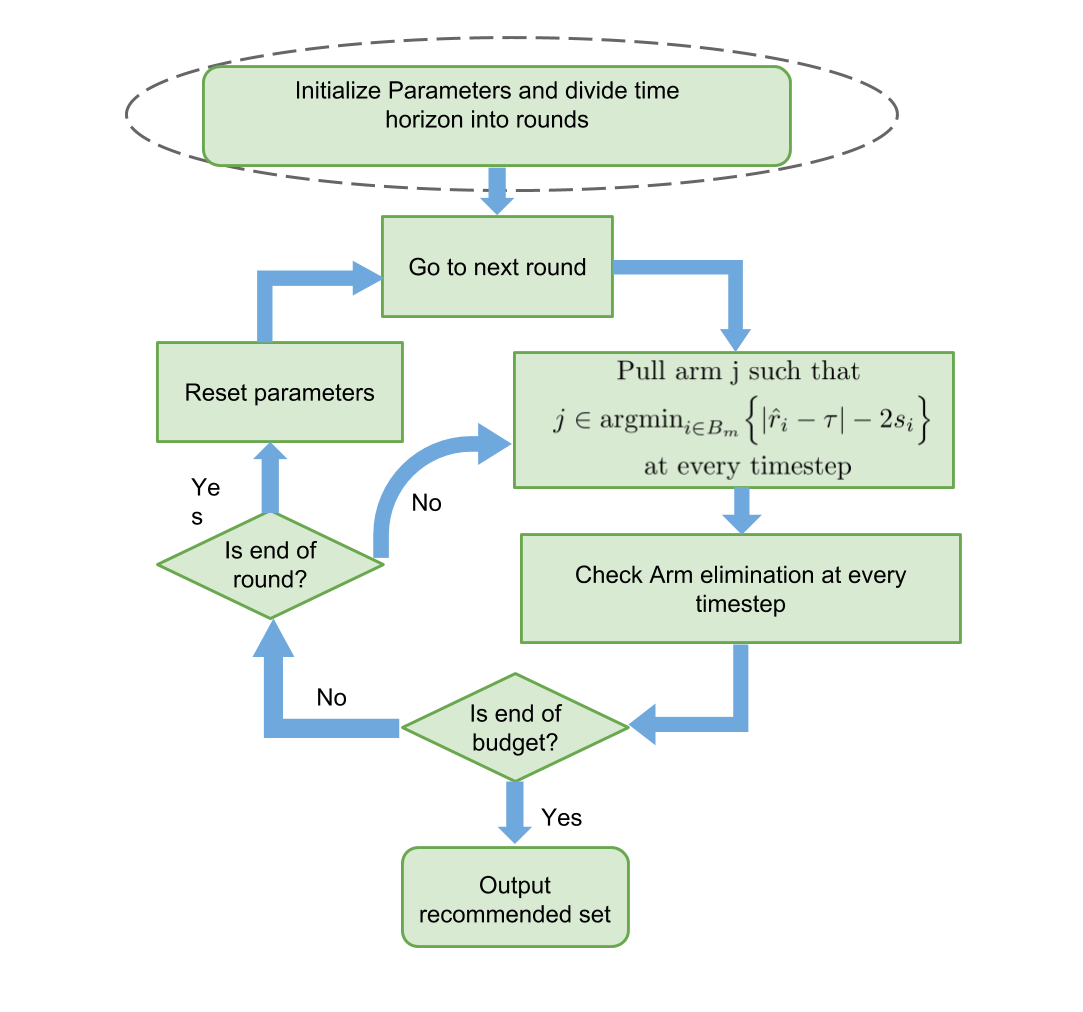
\includegraphics[scale=0.24]{img/AugUCB_flow_param.png}
\end{figure}
\end{frame}


\begin{frame}
\frametitle{Parameter initialization}
\begin{figure}
%\caption{AugUCB parameter initialization}
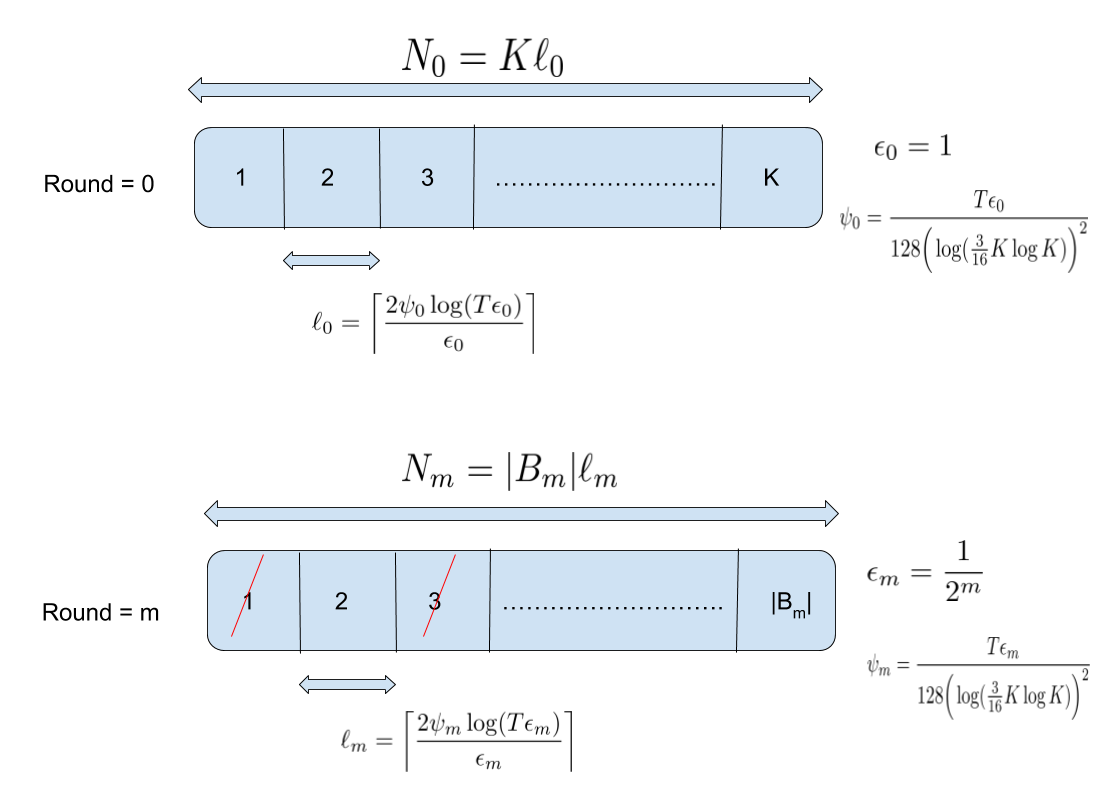
\includegraphics[scale=0.24]{img/InitReset.png}
\end{figure}
%\begin{itemize}
%\item<1-> We define $\ell_{0} =\left\lceil \frac{2\psi_0\log( T\epsilon_{0})}{\epsilon_{0}} \right\rceil$ as the budget allocated to each arm in a round.
%\item<2-> The first round gets divided into $N_{0}=K\ell_{0}$ timesteps.
%\item<3-> We define a large exploration regulatory factor $\psi_{0}=\frac{T\epsilon_{0}}{128\Big(\log(\frac{3}{16}K\log K)\Big)^2}$ which controls exploration.
%\end{itemize}
\end{frame}

\begin{frame}
\frametitle{AugUCB arm pull}
\begin{figure}
%\caption{AugUCB arm pulln}
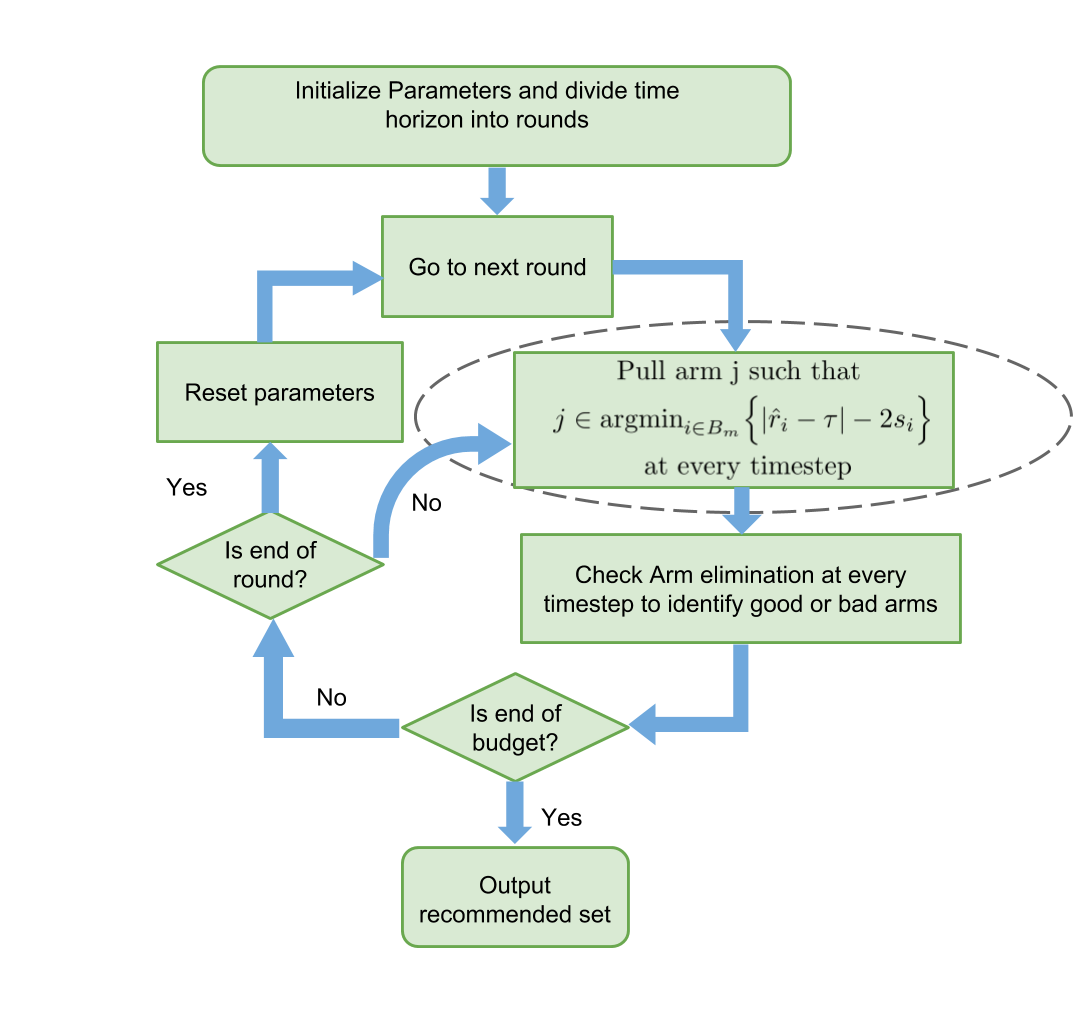
\includegraphics[scale=0.24]{img/AugUCB_flow_armpull.png}
\end{figure}
\end{frame}

\begin{frame}
\frametitle{Arm pull}
\begin{itemize}
\item<1-> We pull the arm that minimizes $j\in\argmin_{i\in B_{m}}\Big\lbrace |\hat{r}_{i} - \tau | - 2s_{i}\Big\rbrace$
\item<2-> We define the confidence interval $s_i  = \sqrt{\frac{\rho\psi_m (\hat{v}_{i}+1) \log ( T \epsilon_{m})}{4 n_{i}}}$.
\item<3-> $s_i$ decreases with more $n_i$ and $\psi_m$ and $\rho$ ensures that it decreases at a correct rate.
\item<4-> Note that $\hat{v}_i$ estimated variance in $s_i$ makes the algorithm pull the arm which shows more variance. 
\end{itemize}
\end{frame}

\begin{frame}
\frametitle{AugUCB arm elimination}
\begin{figure}
%\caption{AugUCB arm elimination}
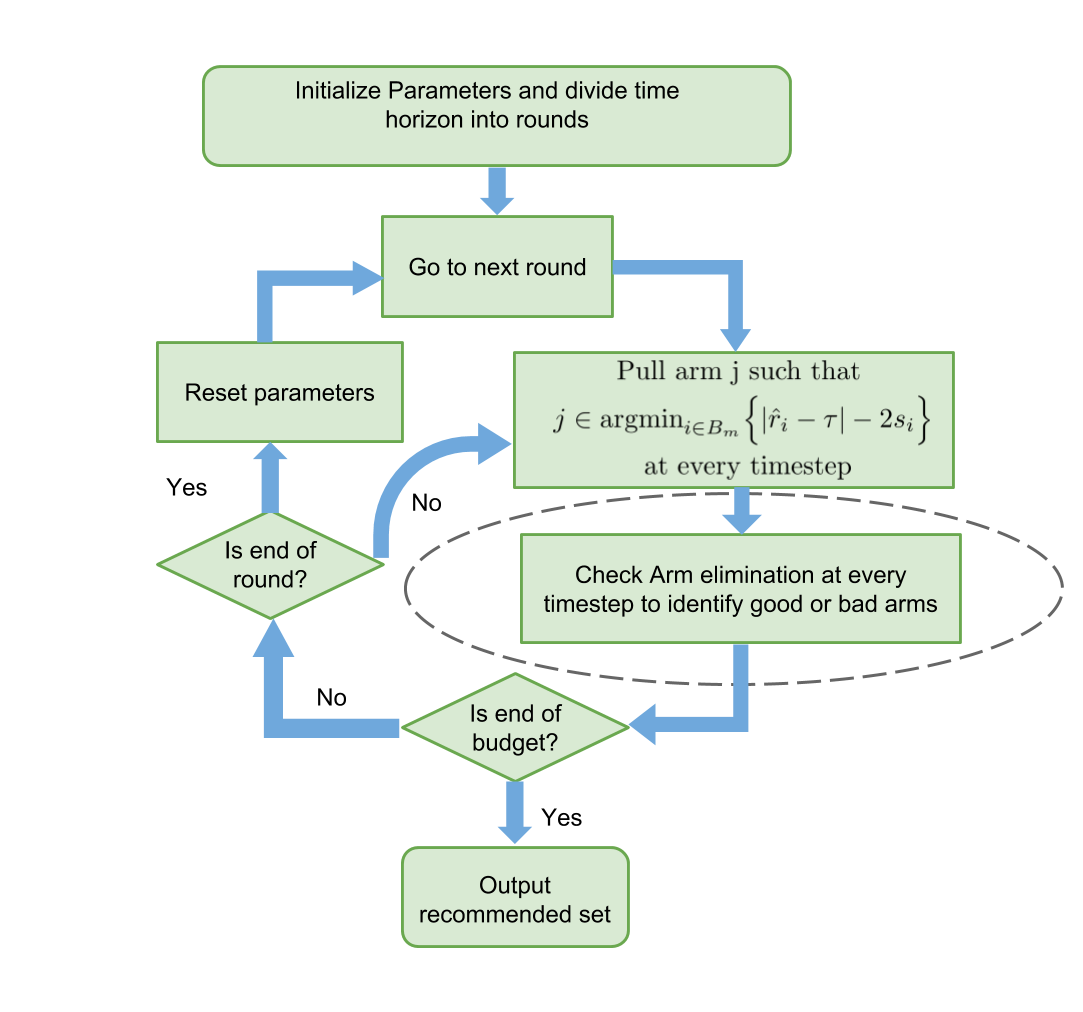
\includegraphics[scale=0.24]{img/AugUCB_flow_elim.png}
\end{figure}
\end{frame}


\begin{frame}
\frametitle{Arm elimination}
\begin{itemize}
\item<1-> Arm elimination condition is checked at every timestep.
\item<2-> It eliminated arm which are above or below margin.
\item<3-> Re-allocates the remaining budget for surviving arms. 
\end{itemize}
\end{frame}


\begin{frame}
\frametitle{AugUCB parameter reset}
\begin{figure}
%\caption{AugUCB parameter reset}
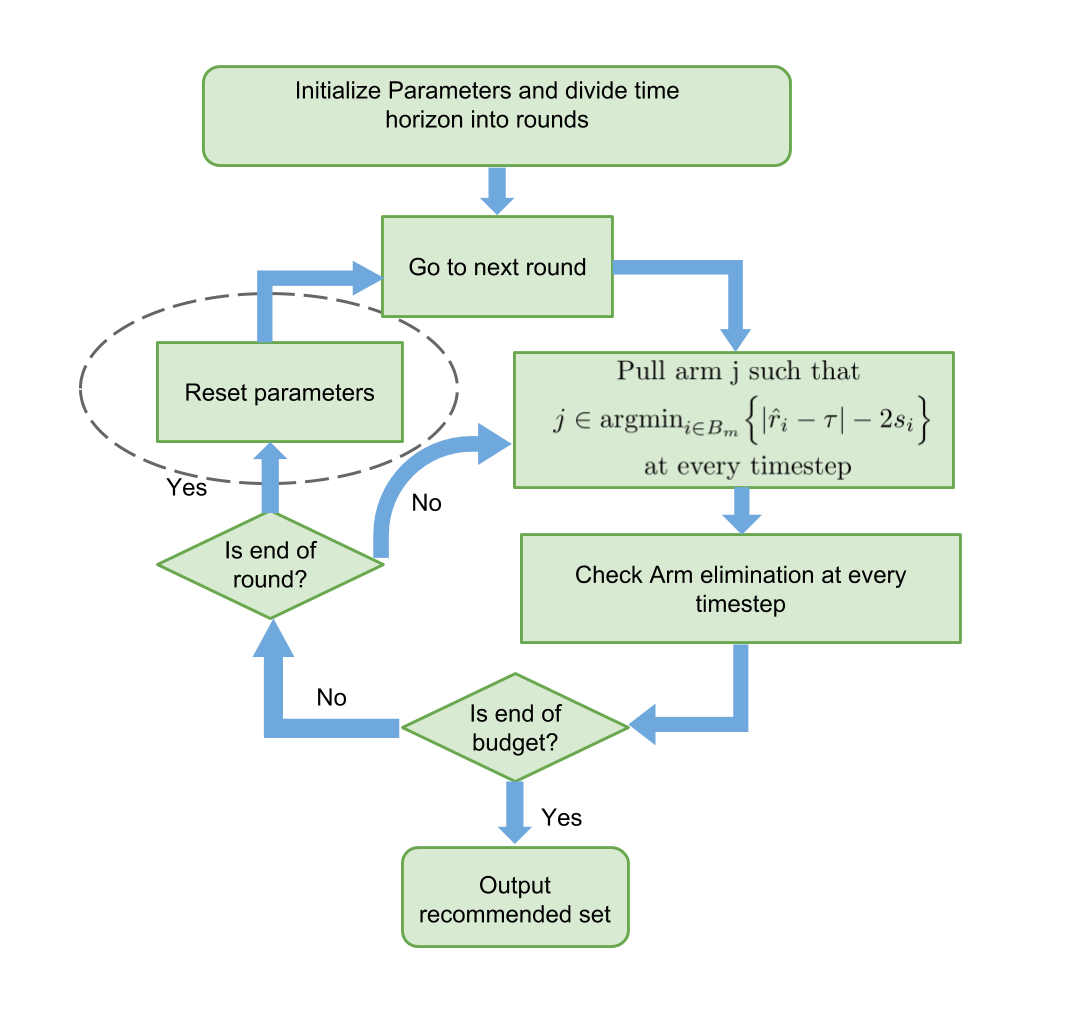
\includegraphics[scale=0.24]{img/AugUCB_flow_reset.png}
\end{figure}
\end{frame}


\begin{frame}
\frametitle{AugUCB parameter reset}
\begin{itemize}
\item<1-> Increase the allocated pulls $\ell_m$ for each surviving arms.
\item<2-> Proportionally reduce the exploration factor $\psi_m$ for next round.
%\item<2-> Recalculate the budget for each surviving arms.
\item<3-> Recalculate the length of next round on the number of surviving arms.
\end{itemize}
\end{frame}

%\begin{frame}[allowframebreaks]
%\frametitle{AugUCB algorithm}
%%\begin{algorithm}[H]
%%\caption{AugUCB}
%%\label{alg:augucb}
%\begin{algorithmic}
%\State {\bf Input:} Time budget $T$; parameter $\rho$; threshold $\tau$
%\State {\bf Initialization:} $B_{0}=\mathcal{A}$; $m=0$; $\epsilon_{0}=1$;
%\begin{small}
%\begin{align*}
%M&=\left\lfloor \frac{1}{2}\log_{2} \frac{T}{e}\right\rfloor; 
%\hspace{2mm}\psi_{0}=\frac{T\epsilon_{0}}{128\Big(\log(\frac{3}{16}K\log K)\Big)^2}; \\
%\ell_{0}&=\left\lceil \frac{2\psi_0\log( T\epsilon_{0})}{\epsilon_{0}} \right\rceil ;
%\hspace{2mm}N_{0}=K\ell_{0}
%\end{align*}
%\end{small}
%\State Pull each arm once
%\vspace{-3mm}
%\State \For{$t=K+1,..,T$}
%\State Pull arm $j\in\argmin_{i\in B_{m}}\Big\lbrace |\hat{r}_{i} - \tau | - 2s_{i}\Big\rbrace$
%\vspace{-4.5mm}
%\State \For{$i\in B_m$}
%\vspace{-4.5mm}
%\State \If{$(\hat{r}_{i} + s_i  < \tau - s_i)$ or $(\hat{r}_{i} - s_i > \tau + s_i)$}
%\State $B_m\leftarrow B_m\backslash\{i\}$\hspace{4mm} (Arm deletion)
%\EndIf
%\EndFor
%\vspace{-2mm}
%\State \If{$t\geq N_{m}$ and $m \leq M$}
%%\ResetParam
%\State \textbf{Reset Parameters}
%\State $\epsilon_{m+1}\leftarrow\frac{\epsilon_{m}}{2}$
%\State $B_{m+1} \leftarrow B_{m}$
%\State $\psi_{m+1}\leftarrow \frac{T\epsilon_{m+1}}{128(\log(\frac{3}{16}K\log K))^{2}}$
%\State $\ell_{m+1}\leftarrow\left\lceil \frac{2\psi_{m+1}\log( T\epsilon_{m+1})}{\epsilon_{m+1}} \right\rceil$
%\State $N_{m+1} \leftarrow t + |B_{m+1}|\ell_{m+1}$
%\State $m \leftarrow m+1$
%\EndIf
%\EndFor
%\State \textbf{Output:} $\hat{S}_{\tau}=\lbrace i: \hat{r}_{i}\geq \tau \rbrace$.
%\end{algorithmic}
%%\end{algorithm}
%\end{frame}

\section{Theoretical Analysis}
\begin{frame}
\frametitle{Problem Complexity}
\begin{itemize}
\item<1-> We must delve into the notion of hardness which come from the general pure exploration bandit literature.
\item<2-> We define $H_{1} = \sum_{i=1}^{K}\dfrac{1}{\Delta_{i}^{2}}$ and $
H_{2} =\min_{i\in \mathcal{A}}\dfrac{i}{{\Delta_{(i)}^{2}}} $ where $\Delta_{(i)}$ is an increasing ordering of ${\Delta}_{i}$.
%\end{align*}$
%where $(\Delta_{(i)}: i\in\mathcal{A})$ is obtained by arranging $(\Delta_i:i\in\mathcal{A})$ in an increasing order. Also, from \cite{chen2014combinatorial} we have
%\begin{align*}
%H_{CSAR,2}=\max_{i\in\mathcal{A}}\frac{i}{\Delta_{(i)}^2}.
%\end{align*}
%$H_{CSAR,2}$ is the complexity term appearing in the bound for the CSAR algorithm. The relation between the above complexity terms are as follows (see \cite{locatelli2016optimal}):
%
%$H_1$ and $H_2$ is same as the problem complexity defined in \cite{locatelli2016optimal} for the thresholding bandit problem while $H_{CSAR,2}=\max_{i}\frac{i}{\Delta_{(i)}^2}$ is defined in \cite{chen2014combinatorial}. Also we know from \cite{locatelli2016optimal} that,
\item<3-> The relationship between $H_1$ and $H_2$ can be derived as,
\begin{align*}
H_{2} \leq H_{1}\leq \log(2K)H_{2} 
%\mbox{ and }
 %H_1 \leq \log(K)H_{CSAR,2}.
\end{align*}
\end{itemize}
\end{frame}

\begin{frame}
\frametitle{Problem Complexity}
\begin{itemize}
\item<1-> For a variance aware algorithm we define $H_{\sigma , 1}$ ( as in {Gabillon et al. (2011)}) that incorporates reward variances into its expression as:
\begin{align*}
 H_{\sigma,1}=\sum_{i=1}^{K}\frac{\sigma_{i}+\sqrt{\sigma_{i}^{2}+(16/3)\Delta_{i}}}{\Delta_{i}^{2}}.
\end{align*}

\item<2-> Finally, analogous to $H_{2}$, we introduce $H_{\sigma,2}$, such that $
H_{\sigma,2}=\max_{i\in \mathcal{A}} \frac{i}{\tilde{\Delta}_{(i)}^{2}}$ , where $\tilde{\Delta}_{i}^{2}=\frac{\Delta_{i}^{2}}{\sigma_{i}+\sqrt{\sigma_{i}^{2}+(16/3)\Delta_{i}}}$,  $(\tilde{\Delta}_{(i)})$ is an increasing ordering of $(\tilde{\Delta}_{i})$.

\item<3-> From \cite{audibert2010best}, we can show that
\begin{align*}
H_{\sigma,2}\le H_{\sigma,1} \le \log(2K) H_{\sigma,2}.
\end{align*}


\item<4-> Note that $H_1 , H_2 $ and $H_{\sigma,1}, H_{\sigma,2}$ are not directly comparable to each other except in a special case when variances are very low we can say that $H_{\sigma,1} < H_{1} $.

\end{itemize}
\end{frame}



\begin{frame}
\frametitle{Expected Loss of AugUCB}

\begin{theorem}
For $K\geq 4$ and $\rho={1}/{3}$,
the expected loss of the AugUCB algorithm is given by,
\begin{align*}
\E[\Ls(T)]
& \leq 2KT \exp\bigg(- \frac{T}{4096 \log( K\log K) H_{\sigma,2}} \bigg).
\end{align*}
\end{theorem}


\begin{table}[b]
\caption{AugUCB vs.\ State of the art}
\label{tab:regret-bds}
\begin{center}
\begin{tabular}{|p{1.5cm}|p{6.4cm}|}
% \toprule
\hline
Algorithm  & Upper Bound on Expected Loss \\
% \midrule
\hline
%\hline
AugUCB      &$ \exp\left(- \frac{T}{4096 \log(K\log K)H_{\sigma,2}} + \log\left(2KT\right) \right) $ \\
%\hline
\hline
UCBEV		&$\exp\left(-\frac{1}{512}\frac{T-2K}{H_{\sigma,1}} + \log\left(6KT\right)\right)$ \\
%\midrule
%\hline
\hline
APT         &$\exp\left(-\frac{T}{64 H_1}+2\log((\log(T)+1)K)\right)$ \\
% \midrule
%\hline
\hline
CSAR		&$\exp\left(-\frac{T-K}{72\log(K)H_{CSAR,2}}+2\log(K)\right)$ \\
%\midrule
\hline

%\bottomrule
\end{tabular}
\end{center}
\end{table}
\end{frame}

%\begin{frame}
%\frametitle{Concentration Bounds}
%\begin{itemize}
%\item<1-> Let $X_{1}, . . . , X_{n}$ be random variables with common support $[0, 1]$ and such that $E[X_{t} |X_{1}, . . . , X_{t-1}] = r_i$. Let $\hat{r}_i = \dfrac{X_{1} +,....,+ X_{n}}{n}$. Then for all $c \geq 0$,
%\begin{align*}
%\mathbb{P} \lbrace \hat{r}_i \geq r_i + c \rbrace \leq \exp{(-2c^{2}n)}\\
%\mathbb{P}\lbrace \hat{r}_i \leq r_i - c \rbrace \leq \exp{(-2c^{2}n)}
%\end{align*}
%
%\item<2-> Along with the above information if we know that $\text{Var}[X_{t} |X_{1}, . . . , X_{t-1}]=\sigma_i^2$ then Bernstein inequality gives us,
%\begin{align*}
%\mathbb{P} \lbrace \hat{r}_i \geq r_i + c \rbrace \leq \exp{(-\dfrac{c^{2}n}{2\sigma_i^2 +\frac{2c}{3}})}\\
%\mathbb{P}\lbrace \hat{r}_i \leq r_i - c \rbrace \leq \exp{(-\dfrac{c^{2}n}{2\sigma_i^2 +\frac{2c}{3}})}
%\end{align*}
%
%\end{itemize}
%\end{frame}

\begin{frame}
\frametitle{Sketch of the proof}
\begin{itemize}
\item<1-> The proof comprises of two modules. In the first module we investigate the necessary conditions for arm elimination within a specified number of rounds, which is motivated by the technique in UCB-Imp. 
 
\item<2-> We bound the arm-elimination probability by Bernstein inequality (as in {Audibert et al. (2009)}) rather that the Chernoff-Hoeffding bounds (used in UCB-Imp). 

\item<3-> In the second module,we define a favourable event that will yield an upper bound on the expected loss and use union bound and module-1 (on the arm elimination probability) to derive the result through a series of simplifications.
\end{itemize}

\end{frame}





\section{Experiments}
%\begin{frame}
%\frametitle{Finally, experiment!!!}
%\begin{figure}[tbp]
%    \centering
%    \begin{tabular}{cc}
%    \subfigure[0.32\textwidth][Expt-$1$: Arithmetic Progression (Gaussian)]
%    {
%    		\pgfplotsset{
%		tick label style={font=\Large},
%		label style={font=\Large},
%		legend style={font=\Large},
%		}
%        \begin{tikzpicture}[scale=0.5]
%      	\begin{axis}[
%		xlabel={Time-step},
%		ylabel={Error Percentage},
%		grid=major,
%        %clip mode=individual,grid,grid style={gray!30},
%        clip=true,
%        %clip mode=individual,grid,grid style={gray!30},
%  		legend style={at={(0.5,1.2)},anchor=north, legend columns=3} ]
%      	% UCB
%		\addplot table{results/budgetTestAP/APT12_comp_subsampled.txt};
%		\addplot table{results/budgetTestAP/AugUCBV1_comp_subsampled.txt};
%		%\addplot table{results/budgetTestAP/AugUCBV_1_13_comp_subsampled.txt};
%		\addplot table{results/budgetTestAP/UCBEM1_comp_subsampled.txt};
%		\addplot table{results/budgetTestAP/UCBEMV1_comp_subsampled.txt};
%		\addplot table{results/budgetTestAP/SR1_comp_subsampled.txt};
%		\addplot table{results/budgetTestAP/UA1_comp_subsampled.txt};
%		%\addplot table{results/budgetTestAP/AugUCBM12_comp_subsampled.txt};
%		%\addplot table{results/budgetTestAP/AugUCBV1_comp_subsampled.txt};
%      	%\legend{APT,AugUCB,UCBE,UCBEV,CSAR,Unif Alloc,AugUCBM,AugUCBV}
%      	\legend{APT,AugUCB,UCBE,UCBEV,CSAR,UA}
%      	\end{axis}
%      	\end{tikzpicture}
%  		\label{Fig:budgetExpt1}
%    }
%    &
%    \subfigure[0.32\textwidth][Expt-$2$: Geometric Progression (Gaussian)]
%    {
%    	\pgfplotsset{
%		tick label style={font=\Large},
%		label style={font=\Large},
%		legend style={font=\Large},
%		}
%        \begin{tikzpicture}[scale=0.5]
%        \begin{axis}[
%		xlabel={Time-step},
%		ylabel={Error Percentage},
%        %clip mode=individual,grid,grid style={gray!30},
%		grid=major,
%		clip=true,
%  		legend style={at={(0.5,1.2)},anchor=north, legend columns=3} ]
%        % UCB
%		\addplot table{results/budgetTestGP/APT12_comp_subsampled.txt};
%		\addplot table{results/budgetTestGP/AugUCBV1_comp_subsampled.txt};
%		%\addplot table{results/budgetTestGP/AugUCBV_1_13_comp_subsampled.txt};
%		\addplot table{results/budgetTestGP/UCBEM1_comp_subsampled.txt};
%		\addplot table{results/budgetTestGP/UCBEMV1_comp_subsampled.txt};
%		\addplot table{results/budgetTestGP/SR1_comp_subsampled.txt};
%		\addplot table{results/budgetTestGP/UA1_comp_subsampled.txt};
%		%\addplot table{results/budgetTestGP/AugUCBM12_comp_subsampled.txt};
%		%\addplot table{results/budgetTestGP/AugUCBV1_comp_subsampled.txt};
%        %\legend{APT,AugUCB,UCBE,UCBEV,CSAR,Unif Alloc,AugUCBM,AugUCBV}
%        \legend{APT,AugUCB,UCBE,UCBEV,CSAR,UA}
%      	\end{axis}
%      	\label{Fig:budgetExpt2}
%        \end{tikzpicture}
%    }
%    \end{tabular}
%\end{figure}
%\end{frame}
%
%\begin{frame}
%\frametitle{Finally, experiment!!!}
%\begin{figure}[tbp]
%    \centering
%    \begin{tabular}{cc}
%    \subfigure[0.32\textwidth][Expt-$3$: Three Group Setting (Gaussian)]
%    {
%    		\pgfplotsset{
%		tick label style={font=\Large},
%		label style={font=\Large},
%		legend style={font=\Large},
%		}
%        \begin{tikzpicture}[scale=0.5]
%        \begin{axis}[
%		xlabel={Time-step},
%		ylabel={Error Percentage},
%        %clip mode=individual,grid,grid style={gray!30},
%       	grid=major,
%       	clip=true,
%  		legend style={at={(0.5,1.2)},anchor=north, legend columns=3} ]
%      	% UCB
%		\addplot table{results/budgetTestGR1/APT1_comp_subsampled.txt};
%		\addplot table{results/budgetTestGR1/AugUCB1_comp_subsampled.txt};
%		\addplot table{results/budgetTestGR1/UCBEM1_comp_subsampled.txt};
%		\addplot table{results/budgetTestGR1/UCBEMV1_comp_subsampled.txt};
%		\addplot table{results/budgetTestGR1/SR1_comp_subsampled.txt};
%		\addplot table{results/budgetTestGR1/UA1_comp_subsampled.txt};
%        \legend{APT,AugUCB,UCBE,UCBEV,CSAR,UA}
%      	\end{axis}
%      	\end{tikzpicture}
%   		\label{Fig:budgetExpt3} 
%    }
%    &
%    \subfigure[0.32\textwidth][Expt-$4$: Two Group Setting (Gaussian) ]
%    {
%    	\pgfplotsset{
%		tick label style={font=\Large},
%		label style={font=\Large},
%		legend style={font=\Large},
%		}
%        \begin{tikzpicture}[scale=0.5]
%        \begin{axis}[
%		xlabel={Time-step},
%		ylabel={Error Percentage},
%        %clip mode=individual,grid,grid style={gray!30},
%		grid=major,
%		clip=true,
%  		legend style={at={(0.5,1.2)},anchor=north, legend columns=3} ]
%        % UCB
%		\addplot table{results/budgetTestGR2/APT1_comp_subsampled.txt};
%		\addplot table{results/budgetTestGR2/AugUCBV1_comp_subsampled.txt};
%		%\addplot table{results/budgetTestGP/AugUCBV_1_13_comp_subsampled.txt};
%		\addplot table{results/budgetTestGR2/UCBEM1_comp_subsampled.txt};
%		\addplot table{results/budgetTestGR2/UCBEMV1_comp_subsampled.txt};
%		\addplot table{results/budgetTestGR2/SR1_comp_subsampled.txt};
%		\addplot table{results/budgetTestGR2/UA1_comp_subsampled.txt};
%		%\addplot table{results/budgetTestGP/AugUCBM12_comp_subsampled.txt};
%		%\addplot table{results/budgetTestGP/AugUCBV1_comp_subsampled.txt};
%        %\legend{APT,AugUCB,UCBE,UCBEV,CSAR,Unif Alloc,AugUCBM,AugUCBV}
%        \legend{APT,AUgUCB,UCBE,UCBEV,CSAR,UA}
%        %\legend{APT,AugUCB,UCBE,UCBEV,CSAR,Unif Alloc}
%      	\end{axis}
%      	\label{Fig:budgetExpt4}
%        \end{tikzpicture}
%    }
%	\end{tabular}
%\end{figure}
%\end{frame}    
%    


\begin{frame}
\frametitle{Finally, experiment!!!}
\begin{itemize}
\item<1-> We compare with APT, AugUCB, UCBE, UCBEV, CSAR, UA.
\item<2-> Note that UCBE and UCBEV require access to $H_1$ and $H_{\sigma, 1}$ as input and hence not implementable in real life. 
\item<2-> By access we mean that an oracle supplies them the $H_1$ or $H_{\sigma, 1}$. They do not have access to individual means and variances.
\item<3-> APT, AugUCB, CSAR, UA do not require access to $H_1$ or $H_{\sigma, 1}$.
\item<4-> UCBE, UCBEV, CSAR and UA come from the pure exploration lineage and are modified suitably to perform in TBP setting.
\end{itemize}
\end{frame}

\begin{frame}
\frametitle{Experimental Setup}
\begin{itemize}
\item<1-> This setup involves Gaussian reward distributions with $K=100, T=10000$ and $\tau=0.5$ with the reward means set in two groups.
\item<2-> The first $10$ arms partitioned into two groups; the respective means are $r_{1:5}=0.45$, $r_{6:10}=0.55$.
\item<3-> The means of arms $i=11:100$ are chosen same as $r_{11:100}=0.4$.
\item<3-> Variances are set as $\sigma_{1:5}^{2}=0.3$ and $\sigma_{6:10}^{2}=0.8$;  $\sigma_{11:100}^{2}$ are independently and uniformly chosen in the interval $[0.2,0.3]$. 
\end{itemize}
\end{frame}


\begin{frame}
\frametitle{Experimental Result}
\begin{figure}[tbp]
    \centering
    \begin{tabular}{cc}
    \subfigure[0.32\textwidth][Expt-$1$: Two Group Setting (Advance) ]
    {
    	\pgfplotsset{
		tick label style={font=\Large},
		label style={font=\Large},
		legend style={font=\Large},
		}
        \begin{tikzpicture}[scale=0.5]
        \begin{axis}[
		xlabel={Time-step},
		ylabel={Error Percentage},
        %clip mode=individual,grid,grid style={gray!30},
		grid=major,
		clip=true,
  		legend style={at={(0.5,1.2)},anchor=north, legend columns=3} ]
        % UCB
		\addplot table{results/budgetTestGR4/APT1_comp_subsampled.txt};
		\addplot table{results/budgetTestGR4/AugUCB1_comp_subsampled.txt};
		\addplot table{results/budgetTestGR4/UCBEM1_comp_subsampled.txt};
		\addplot table{results/budgetTestGR4/UCBEMV1_comp_subsampled.txt};
		\addplot table{results/budgetTestGR4/SR1_comp_subsampled.txt};
		\addplot table{results/budgetTestGR4/UA1_comp_subsampled.txt};
        \legend{APT,AugUCB,UCBE,UCBEV,CSAR,UA}
      	\end{axis}
      	\label{Fig:budgetExpt5}
        \end{tikzpicture}
    }
    &
    \subfigure[0.32\textwidth][Expt-$2$: Two Group Setting (Advance) ]
    {
    	\pgfplotsset{
		tick label style={font=\Large},
		label style={font=\Large},
		legend style={font=\Large},
		}
        \begin{tikzpicture}[scale=0.5]
        \begin{axis}[
		xlabel={Time-step},
		ylabel={Error Percentage},
        %clip mode=individual,grid,grid style={gray!30},
		grid=major,
		clip=true,
  		legend style={at={(0.5,1.2)},anchor=north, legend columns=2} ]
        % UCB
		\addplot table{results/budgetTestGR3/testUCBEMV1_0.25_comp_subsampled.txt};
		\addplot table{results/budgetTestGR4/AugUCB1_comp_subsampled.txt};
		%\addplot table{results/budgetTestGP/AugUCBV_1_13_comp_subsampled.txt};
		%\addplot table{results/budgetTestGR3/testUCBEMV1_0.25_comp_subsampled.txt};
		\addplot table{results/budgetTestGR3/testUCBEMV1_256_comp_subsampled.txt};
		\addplot table{results/budgetTestGR4/UCBEMV1_comp_subsampled.txt};
		%\addplot table{results/budgetTestGR3/testUCBEMV1_64_comp_subsampled.txt};
		%\addplot table{results/budgetTestGP/AugUCBM12_comp_subsampled.txt};
		%\addplot table{results/budgetTestGP/AugUCBV1_comp_subsampled.txt};
        %\legend{APT,AugUCB,UCBE,UCBEV,CSAR,Unif Alloc,AugUCBM,AugUCBV}
        \legend{UCBEV($0.25$), AugUCB, UCBEV($256$), UCBEV($1$)}
        %\legend{UCBEV($0.06$),AUgUCB,UCBEV($0.25$),UCBEV($1$),UCBEV($64$),UCBEV($256$)}
        %\legend{APT,AugUCB,UCBE,UCBEV,CSAR,Unif Alloc}
      	\end{axis}
      	\label{Fig:budgetExpt6}
        \end{tikzpicture}
    }
    \end{tabular}
\end{figure}
\end{frame}

\section{Conclusion}
\begin{frame}
\frametitle{Conclusion}
\begin{itemize}
\item<1-> We proposed the AugUCB algorithm for the fixed budget TBP  which uses variance estimation and arm elimination to give an improved theoretical and experimental guarantees than APT.
\item<1-> This work has been accepted in the proceedings of IJCAI 2017. I thank my collaborator Dr. K.P. Naveen and both my guides for guiding me through this work.
\item<2-> Further studies are required to establish a lower bound on the expected loss of AugUCB.
\item<3-> A more detailed analysis of the non-uniform arm selection and parameter selection is also required.
\end{itemize}
\end{frame}

%\begin{frame}
%\frametitle{Future direction in MS}
%\begin{itemize}
%\item<1-> This work has been accepted in IJCAI 2017.
%\item<2-> We have proposed a very similar algorithm as like AugUCB for the SMAB (single best arm) problem with more detailed study of non-uniform arm selection and parameter selection.
%\item<3-> Termed as Efficient UCBV, we are preparing for submission for AAAI 2018.
%\item<4-> I am going to INRIA, SequeL Lab, Lille, France for a three month internship starting from 1st September under Dr. Odalric Maillard.
%\end{itemize}
%\end{frame}

%\begin{frame}
%\frametitle{Future direction in MS}
%\Huge{\centerline{Any Questions? }}
%
%\end{frame}

\section{References}
\begin{frame}[allowframebreaks]
\frametitle{References}
%\bibliographystyle{named} 
\bibliographystyle{plainnat} 
%\bibliographystyle{dinat}
\bibliography{ijcai17}
\end{frame}


%------------------------------------------------

\begin{frame}
\Huge{\centerline{Thank You}}
\end{frame}

%----------------------------------------------------------------------------------------

\end{document} 